\subsection{LETs based on carbon nanotubes} %Armin|Cees

%LET OP: de ~ is voor latex, zo vertellen we dat de punt niet een einde-van-de-zin-punt is maar een afkortingspunt, oftewel niet extra ruimte voor een nieuwe zin invoegen (want erna volgt niet een nieuwe zin).

To prepare nanoscale light sources for use in fully integrated opto-electronic circuits, there are several methods. One of them is the engineering of light-emitting nanowires made of direct-bandgap semiconductors. Duan et al.\ have made advancements in this field by assembling $p$-doped and $n$-doped nanowires to form a $p$--$n$ junction. Gudiksen et al.~achieved this by fabricating nanowire superlattices. Unfortunately for achieving high performance levels, with these methods ease of fabrication is lost as well. %op zich zou dit hele stuk weg kunnen omdat het niet direct over carbon nanotubes gaat, maar over nanowires.

A different approach is to use semiconducting single-walled carbon nanotubes as the active component in a field-effect transistor. Carbon nanotube FETs of $n$-type, $p$-type and ambipolar character have been fabricated. The ambipolar charge transport is achieved by simultaneous injection of holes and electrons via thermally assisted tunnelling through the Schottky barriers formed at the source and drain contacts. Under biasing conditions suitable for ambipolar transport with balanced hole and electron currents, infrared optical emission is generated as the result of electron-hole recombination in the nanotube. This is illustrated in figure~\ref{fig:carbontube}. 

\begin{figure}[!ht]
 \begin{center}
  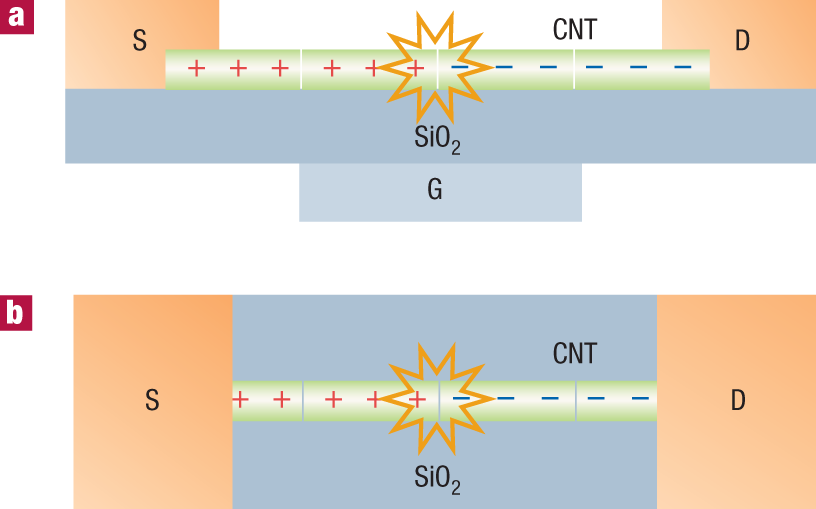
\includegraphics[width=0.6\textwidth]{fig_1}
  \caption{Device structure of a carbon nanotube. (a) Side view. (b) Top view. Infrared emission is generated by the recombination of electrons and holes flowing in the nanotube. From \citet{Muccini}.}
  \label{fig:carbontube}
 \end{center}
\end{figure}

The infrared radiation emitted by the carbon nanotube FET has some special properties. Due to the elongated shape of the tube, the light is polarised parallel to the tube axis. This resembles a linearly polarized dipole radiation source. As the bandgap of the nanotube is inversely proportional to its diameter, it is expected that the wavelength can be tuned by changing diameter sizes. Although this is still to be explored, carbon nanotube LETs offer significant potential as nanoscale photon sources that could easily be integrated in opto-electronic devices.

